\section{Overview}
% Researchers universally assume that participants use the input they receive (i.e., the value of each option) to make a choice.
Decades of decision-making research have shown that context can systematically affect choice. In decision-making experiments, researchers present participants with a finite set of options on each trial and ask them to select a single option based on either an internal (e.g., most preferable) or external (e.g., largest shape) criterion. Decision-making research spans multiple fields, including psychology, neuroscience, economics, marketing, and political science. In economics, for example, researchers have developed models based on the idea that people make choices that maximize their utility but are subject to resource constraints and noisy preferences. In psychology and marketing, however, decision-making researchers have identified a set of phenomena that violate such assumptions, by showing that choices can vary with the \textit{choice set}, or the menu of available options. This class of phenomena is known as \textit{context effects}.

% Context effects are interesting to decision-making researchers because they violate properties exhibited by large classes of choice models, such as Independence of Irrelevant Alternatives (IIA) \parencite{ray1973independence} and regularity \parencite{mackay1995probabilistic,marley1989random}. IIA states that the likelihood of selecting one option over another is invariant of other options available. Regularity states that the probability an option is chosen cannot increase upon the addition of new options to a choice set. IIA and regularity are also properties of Luce's Choice Axiom, a highly influential model of stochastic choice \parencite{luceChoiceAxiomTwenty1977a, luce1959individual}. 

One notable context effect, the attraction effect, occurs when the choice share of a \textit{target} option increases upon the inclusion of a similar but inferior \textit{decoy} option \parencite{huberAddingAsymmetricallyDominated1982d}. Another finding, the repulsion effect, occurs when a decoy boosts the choice share of a dissimilar \textit{competitor} option rather than the target \parencite{simonson2014vices}. The repulsion effect is an empirical reversal of the attraction effect. 

Context effects, originally studied in preferential choice, have been recently demonstrated simple perceptual choice \parencite{trueblood2013not,spektorWhenGoodLooks2018b,liaoInfluenceDistanceDecoy2021,spektorRepulsionEffectPreferential2022,yearsleyContextEffectsSimilarity2022,truebloodPhantomDecoyEffect2017c, turnerCompetingTheoriesMultialternative2018a, evansImpactPresentationOrder2021}. This idea is theoretically interesting because it suggests that context effects are a theoretical primitive rather than simply a feature of high-level consumer choice \parencite{trueblood2013not}. 

As suggested by the title, this dissertation explores various forms of context dependence in both perceptual and preferential choice. Specifically, the dissertation explores the attraction and repulsion effects. The goal of this dissertation is to further understand why these effects occur in perceptual and preferential choice, by employing well-studied statistical models from the psychology literature. Additionally, this dissertation sets out to differentiate perceptual processes from decision-making processes in context effects (specifically, the attraction and repulsion effects).

As discussed throughout this dissertation but particularly in Chapter 2, recent work has demonstrated inconsistency in context effects, particularly in perceptual choice. This dissertation uses behavioral experiments and statistical modeling in an attempt to reconcile these inconsistencies.

This dissertation is structured as follows. Chapter 2, develop and tests a statistical (Thurstonian) model of choice within the domain of perceptual choice. In Experiment 1, it is shown that the types of stimuli used in perceptual choice context effects experiments are easily confusable and vary systematically with theoretically relevant properties of the stimuli. In Experiment 2, the results of a high-powered psychophysics experiment show that the repulsion effect, but not the attraction effect, is naturally predicted by this Thurstonian model. In Chapter 3 further tests the Thurstonian model by applying it to best-worst choice. In Chapter 4 generalizes the paradigm and model to preferential choice. Finally, Chapter 5 uses a perceptual choice experiment to show that stimulus comparability affects choice, even when the decoy is equally similar to both focal options. Chapter 6 summarizes the findings of the dissertation, their implications, and discuss future directions for research in this domain. 

Below, the attraction and repulsion effects are introduced, and the empirical and theoretical literaure is reviewed.

\section{The Attraction Effect}
This section formally defines the attraction effect. See Figure~\ref{fig:fig_opts} (left panel), which shows a graphical configuration of various choice options. These options vary on two dimensions (or attributes), where higher values of an attribute are always preferred. These dimensions are named generically to emphasize the generality of the attraction effect.

Let $A$, $B$, $D_{A}$, and $D_{B}$ be discrete choice options, $[]$ denote the options in a choice set, and $P(A|[A,B])$ denote the probability of choosing option $A$ from a set consisting of $A$ and $B$, for example. 

In Figure~\ref{fig:fig_opts} (left panel), options $A$ and $B$ trade off on attributes. $A$ is high on dimension 2 but low on dimension 1, while $B$ is high on dimension 1 but low on dimension 2. A decision-maker who assigns equal importance to both dimensions should be indifferent between both options when presented with choice set $[A,B]$. Now, however, consider option $D_{A}$, which is inferior to $A$ and $B$, but more similar to $A$ than to $B$. This \textit{decoy} option is dominated by $A$, so no rational agent who perceives this dominance relationship should intentionally select the decoy over the target. Similarly, $D_{B}$ is inferior to both $A$ and $B$ but more similar to $B$. The attraction effect is the finding that choice for $A$ over $B$ is greater given set ${A,B,D_{A}}$ then given set $A,B,D_{B}$. 

% \footnote{This is the weak version of the attraction effect. A strong version requires the ordering of P(A) and P(B) to change with choice set. See \textcite{davis2023illustrated} for a discussion of similar issues.}\parencite{huberAddingAsymmetricallyDominated1982d}. 

\begin{figure}
    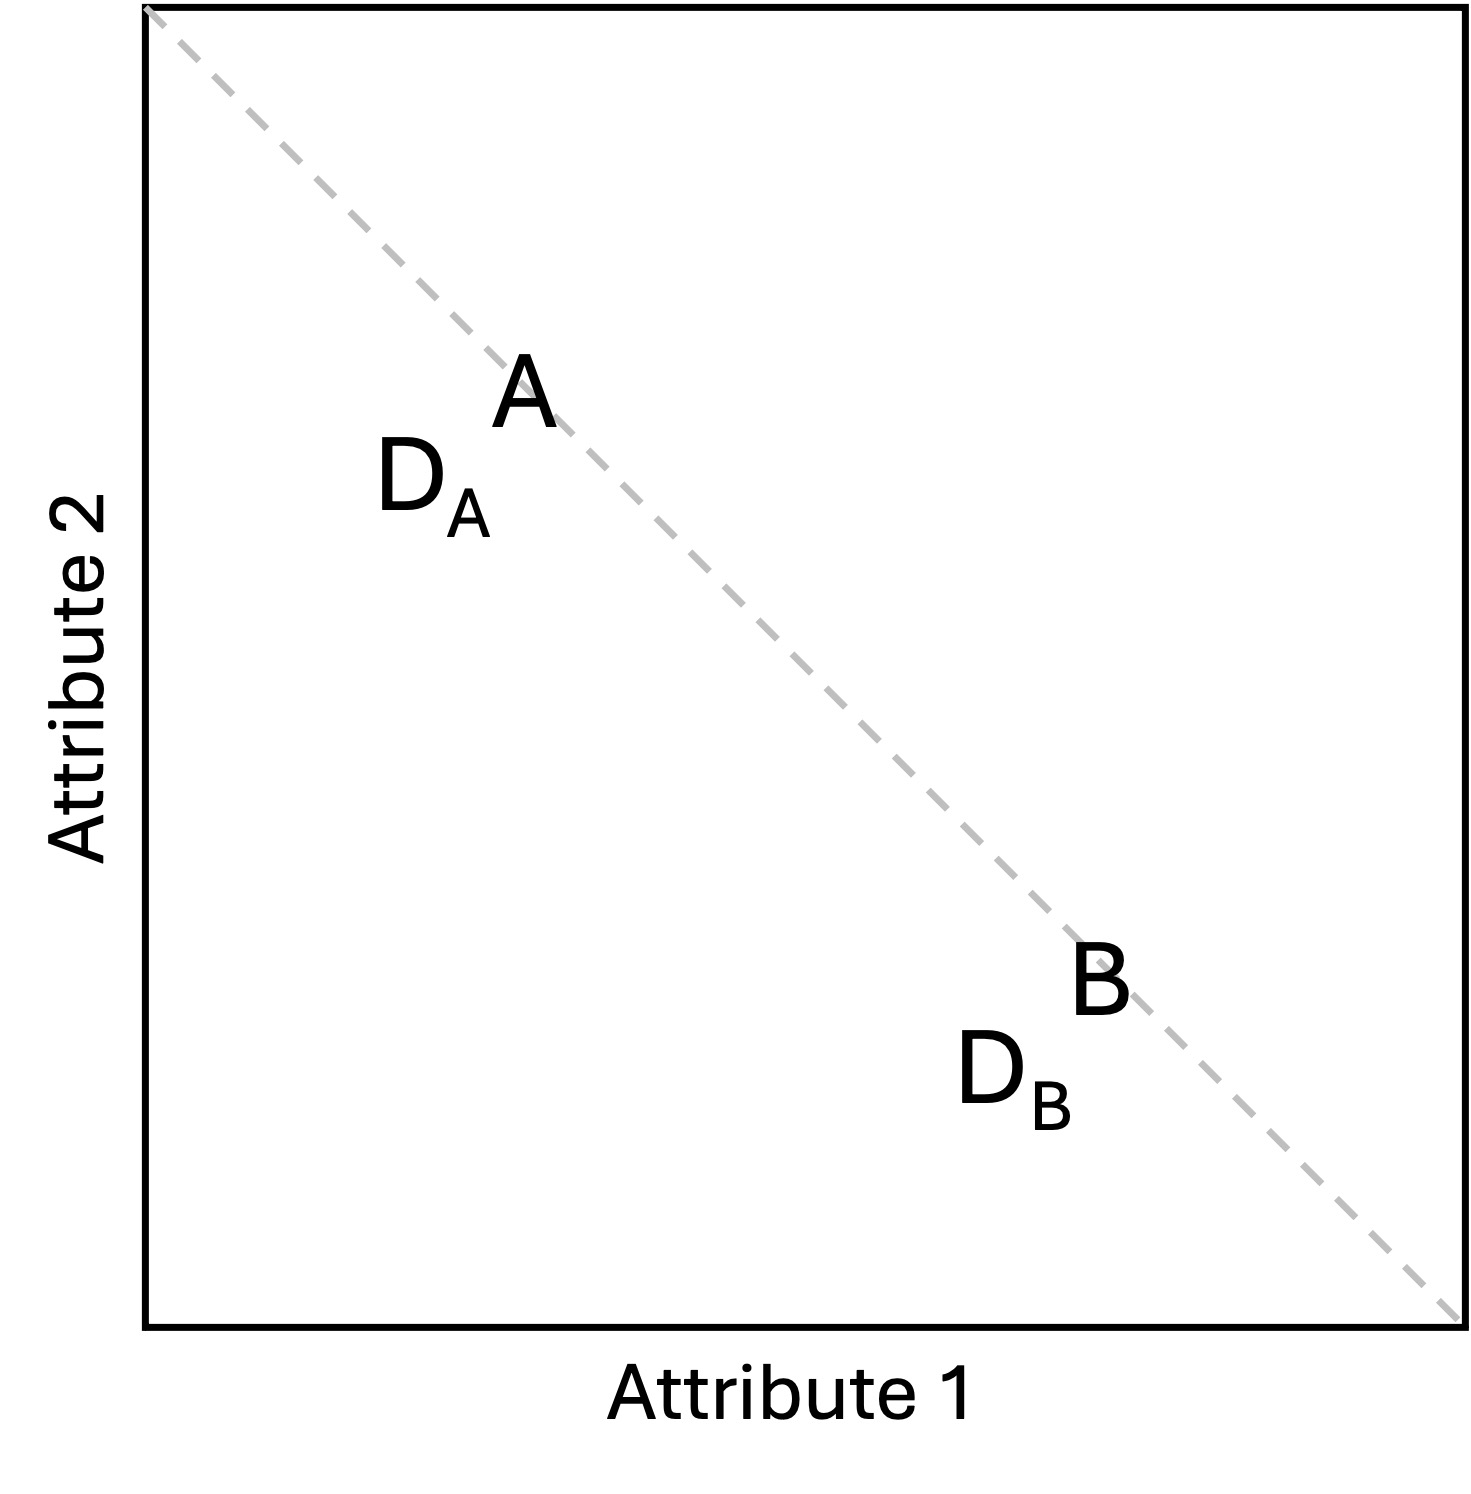
\includegraphics[width=\linewidth]{figures/att_stim.jpg}
   \caption{A graphical depiction of choice options in the attraction/repulsion effect. Attributes are named generically.}
   \label{fig:att_stim}
\end{figure}

The attraction effect was first demonstrated by \textcite{huberAddingAsymmetricallyDominated1982d}\footnote{These authors referred to this finding as the asymmetric dominance effect. Contemporary researchers have adopted the term attraction effect.}, who tested participants with sets of choice options, using products such as cars, beers, and TV sets. Participants first completed hypothetical choice tasks where they chose their most preferred option from ternary choice sets, each containing a target, competitor, and decoy option. Participants then returned two weeks later to choose from the same choice sets but with the decoy removed from all trials. Participants chose the target at a higher proportion when the decoy was present than when it was absent. The results of \textcite{huberAddingAsymmetricallyDominated1982d} violate the regularity principle, which states that the choice proportion for a particular option cannot increase when more options are added to the choice set. According to regularity, the following inequality should hold:

\begin{equation}
  P(A|[A,B])\geq P(A|[A,B,D_{A}])
  \label{eqn:reg_att}
\end{equation}

Thus, the binary-ternary form of the attraction effect demonstrated by \textcite{huberAddingAsymmetricallyDominated1982d}, where $P(A|[A,B,D_{A}])\geq P(A|[A,B])$, violates regularity. 

The attraction effect also violates the \textit{Independence of Irrelevant Alternatives}(IIA) principle. IIA states that the relative likelihood of choosing a particular option over another is invariant of the choice set \parencite{ray1973independence}. 

Written in the context of the above example, IIA requires the follow equality to hold\footnote{This is often referred to as the constant ratio rule.}: 
\begin{equation}
  \frac{P(A|[A,B])}{P(B|[A,B,D_{A}])}=\frac{P(A|[A,B])}{P(B|[A,B,D_{A}])}
  \label{eqn:iia_att}
\end{equation}

However, in the attraction effect, this equality is violated:
\begin{equation}
  \frac{P(A|[A,B,D_{A}])}{P(B|[A,B,D_{A}])}>\frac{P(A|[A,B])}{P(B|[A,B])}
  \label{eqn:iia_att1}
\end{equation}

The attraction effect is often demonstrated by a ternary-ternary comparison \parencite{trueblood2013not}, where participants choose from two choice sets each containing a target, competitor, and decoy option (e.g., $[A,B,D_{A}]$ and  $[A,B,D_{B}]$ in Figure~\ref{fig:att_stim}). In the attraction effect, participants are more likely to choose $A$ given $[A,B,D_{A}]$ than given $[A,B,D_{B}]$, and they are also more likely to choose $B$ given $[A,B,D_{B}]$ than given $[A,B,D_{A}]$. This effect can be written using the following inequality, which also violates IIA:

\begin{equation}
  \frac{P(A|[A,B,D_{A}])}{P(B|[A,B,D_{A}])}>\frac{P(A|[A,B,D_{B}])}{P(B|[A,B,D_{B}])}
  \label{eqn:iia_att2}
\end{equation}

Thus, IIA is violated by the attraction effect in this ternary-ternary example.

In the context effects literature, it is common to refer to the similar, dominated option as the \textit{decoy}, the similar dominating option as the \textit{target}, and the dissimilar dominating option as the \textit{competitor}. For example, in the choice set $[A,B,D_{A}]$, $A$ is the target, $B$ is the competitor, and $D_{A}$ is the decoy. This terminology will be adopted throughout this dissertation.

\textcite{cataldoComparisonProcessAccount2019b} showed that, in preferential choice, context effects can be reversed or eliminated simply by altering stimulus presentation format. For example, they showed that if participants can easily compare pairs of options (e.g., target and decoy) on each dimension, the attraction effect occurs quite strongly, but without this ease of comparison the attraction effect becomes neglible. \textcite{hasan2025registered} failed to replicate this effect, albeit with different decoys than those of \textcite{cataldoComparisonProcessAccount2019b}. 

\textcite{changWhichCompromiseOption2008} also varied option display, in either a by-alternative format, where option names are listed as columns while attribute values are listed as rows, or a by-attribute format, where option attributes are columns while option names are rows. The former display makes it more difficult to compare options on a single attribute, while the latter makes it easier. They found that listing options by-attribute increased the choice share of the compromise option, relative to a by-alternative display. 

\textcite{hayes2024attribute} manipulated attribute commensurability in a context effects experiment. When two dimensions are commensurable, they vary on a common unit (e.g., user ratings from 0-10), while incommensurable units exist on incomparable units (e.g., RAM and CPU speed in laptops). They found that when dimensions are commensurable, the attraction effect vanishes, while it still exists strongly when dimensions are incommensurable. This suggests that the attraction effect occurs more strongly when the representation of options encourages between-option comparisons on a single attribute.

Theoretically, the attraction effect is particularly interesting because in violating IIA and regularity, it is not predicted by many classical models of choice. Luce's Choice Model \parencite{luce1959individual}, for example, is a well-known model of choice which states that the probability of choosing option $x$ from set $K$ can be written as:

\begin{equation}
    P(x|K)=\frac{v_{x}}{\Sigma_{y \in K}v_{y}}
\end{equation}

where $v_{i}$ is a ratio scaled variable indicating value, or utility, of option $i$. Luce's model is highly influential in psychology and has been used to account for data in areas such as categorization \parencite{nosofskyAttentionSimilarityIdentificationCategorization1986} and identification \parencite{townsend1971theoretical}. However, given that the model satisfies both IIA and regularity, the model cannot predict the attraction effect. 

The attraction effect is not the only context effect to be demonstrated empirically; \textcite{tverskyEliminationAspectsTheory1972} demonstrated that a similar, but not necessarily inferior, option can decrease choice for a focal option. For example, an option closer to $A$ than to $B$ on the diagonal line in Figure~\ref{fig:att_stim} can cause a decrease in the choice proportion for $A$. \textcite{simonsonChoiceBasedReasons1989b} demonstrated the compromise effect, where the placement of an intermediate option between two extremes decreases choice for the extremes. 

Context effects such as the attraction effect have strong theoretical implications. Traditional models of choice, as used in economics and marketing research \parencite{mcfadden2001economic}, treat the \textit{utility}, or value, of each option as a random variable whose parameters are estimated from choice data. According to these models, on each trial of a decision-making experiment, the participant samples option values from these distributions and deterministically chooses the option with the highest sampled value. These models are known as \textit{Random Utility Models} (RUMs). When utilities are assumed to follow a Type 1 Generalized Extreme Value distribution, the logit or softmax model is used \parencite{gensch1979multinomial}. The probit model, another popular model, assumes Gaussian distributed utilities \parencite{bolduc1999practical}. Typically, though not necessarily, these models assume independently distributed errors, which typically implies IIA. Typically, these models are used to estimate the inherently unobservable utility values for each option. 

With the large body of published empirical data and the inadequacy of exiting models to explain context effects, many researchers have developed process models that attempt to explain the mental processes that lead to context effects. 

% \textcite{tversky1993context} context-dependent advantage (CDA) model extended utility models to include background contrast (effects of other choice sets that remain in the decision maker’s mind) and all pairwise advantages and disadvantages between options, explaining 

One notable model is \textcite{roeMultialternativeDecisionField2001a}'s Multialternative Decision Field Theory (MDFT) model. Building on other research in cognitive psychology which casts the decision-making process as an evidence accumulation process indexed by time \parencite{ratcliff1978theory}, where evidence here is preference. According to MDFT, the valence \boldsymbol{V} of each option at time $t$ is computed as:

\begin{equation}
    \boldsymbol{V}(t)=\boldsymbol{C}\boldsymbol{M}_1\boldsymbol{W}_1(t) + \boldsymbol{\epsilon}(t)
    \label{eqn:mdft}
\end{equation}

where $\boldsymbol{C}$ is a (symmetric) contrast matrix defining the comparison process, $\boldsymbol{M}$ is a matrix of attribute values, $\boldsymbol{W}$ is a vector of attention weights (defining which attribute is being attended to), and $\epsilon$ is the random error term. 

The valences are then combined into a preference state vector $\boldsymbol{P}(t)$ and a new state is formed at time $t+1$ by:

\begin{equation}
    \boldsymbol{P}(t+1)=\boldsymbol{SP}(t)+\boldsymbol{V}(t+1)
    \label{eqn:mdft1}
\end{equation}

$\boldsymbol{S}$ is a feedback matrix where the diagonal elements allow memory decay for previous preference states, but the off-diagonal elements allow options in a choice set to influence one another through lateral inhibition. \textcite{roeMultialternativeDecisionField2001a} stated that this influence should be negative and its strength should be a decreasing function of distance in attribute space. They did not specify a form to this function, but \textcite{hotalingTheoreticalDevelopmentsDecision2010} amended the model to specify a Gaussian function for the distance, where the value of $\boldsymbol{S}_{ij}$ is computed as:

\begin{equation}
    \boldsymbol{S}_{ij}=\delta_{ij}-\varphi_{2} \cdot e^{-\varphi_{1} \cdot D^2_{ij}}
    \label{eqn:mdft2}
\end{equation}

where $\delta_{ij}=0$ if $i\neq j$ (indicating lateral inhibition), $D^2_{ij}$ is distance in attribute space between options $i$ and $j$\footnote{\textcite{hotalingTheoreticalDevelopmentsDecision2010} also specify that distance should be weighted differently depending on whether one option dominates another.}, and the $\varphi$ are free parameters. 

MDFT can produce the attraction effect because of the strong connection between target and decoy (e.g., $A$ and $B$ in Figure~\ref{fig:att_stim}), where the mutual negative inhibition cancels (via multiplication) to cause the decoy to boost the preference state for the target, relative to the competitor. 

RUMs often have difficulty accounting for context effects. For example, \textcite{berkowitschRigorouslyTestingMultialternative2014b} tested the independent logit and independent probit models against \textcite{roeMultialternativeDecisionField2001a}'s Multialternative Decision Field Theory (MDFT), a cognitive process model of decision-making. According to MDFT, choice is the end result of a stochastic evidence accumulation process, where preferences for each option in a choice set accumulate value through a series of comparisons on each dimension. In \textcite{berkowitschRigorouslyTestingMultialternative2014b}'s experiment participants chose between digital cameras from choice sets designed to elicit context effects. \textcite{berkowitschRigorouslyTestingMultialternative2014b} found that MDFT, but not the logit or probit models, could account for the attraction effect (and other related context effects). Furthermore, according to model comparison measures, the majority of participants were best described by MDFT. Participants whose data were best described by MDFT were also more likely to exhibit context effects. Independent RUMs, such as the logit and probit model, assume each option's utility is independently sampled, so these models cannot account for context effects.

Often, though not necessarily, RUMs assume IIA. This assumption can be relaxed, however. \textcite{paetzUtilityIndependenceIIA2018} showed, via simulations, that the probit model can violate IIA by allowing non-zero off-diagonal elements in the variance-covariance matrix. IIA can also be relaxed by estimating choice set or alternative specific coefficients \parencite{rooderkerk2011incorporating} or allowing correlations between options and/or attributes \parencite{haaijer1998utility}. Without such modifications, RUMs are unable to account for context effects. 

\textcite{huber1983market} replicated the results of \textcite{huber1983market} and also showed that if the decoy has a relatively high value, it can actually take choice shares away from the target. 

% Furthermore, modern psychological models of context effects often assume an attribute-wise comparison process \parencite{roeMultialternativeDecisionField2001a,trueblood2013not,usherLossAversionInhibition2004a,bhatiaAssociationsAccumulationPreference2013b}. Under this class of models, participants arrive at a decision by comparing pairs of options on a single attribute, where the modeller assumes attribute values are veridical. This assumption is quite reasonable when modeling choices where each attribute is presented separately and discriminability issues are minimal or non-existent. In perceptual choice experiments like those presented here or in \textcite{spektorWhenGoodLooks2018b,trueblood2013not}, these assumptions are likely incorrect. However, the general modeling framework, where inter-stimulus comparison leads to preference, which then leads to choice, is still plausible.